
Deep learning is a branch of Machine Learning.

If not specified, vector is column vector by default,
$\sigma()$ denotes sigmoid, $\odot$ denotes element-wise multiplication.

\subsection{Modularized Neural Networks}

 Artificial Neural Networks (ANNs) with cycles are
 referred to as feedback, recursive, or recurrent,
 neural networks. ANNs without cycles are
 referred to as feedforward neural networks (FNNs).
 MLP is the most widely used FNN.

 Feed forward neural network can be trained with the
 BP algorithm. An iteration during training a neural network
 involves four steps: (1) forward pass to get the network output,
 (2) calculate the loss function, (3) backward pass, calculating
 gradient of the loss function {\it w.r.t} the learnable
 parameters, (4) update parameters according to the gradients.
 Recurrent neural networks can be trained with BPTT --
 an extension to the original BP algorithm.

 Modern deep learning frameworks tends to modularize the
 neural networks into individual components like network layers,
 activation functions, loss functions, which brings much
 flexibility for the user.

 During the forward pass of a modularized neural netowrk, the
 modules in the neural network are
 firstly organized as an directed acyclic graph (DAG), and modules
 are processed one by one in the topological order. A module
 recieves input from the previous module(s), and send calculated
 output to module(s) next to it, {\it i.e.} $y=f(x)$. After
 calculating the loss function $E(x,z)$, the backward pass begins.
 In this stage, the modules are processed individually in the
 reversed topological order (See also Reverse Mode Automatic
 Differentiation). A module recieves the gradient of the loss
 function {\it w.r.t} its output from the module(s) next to it,
 {\it i.e.} $\partial E/\partial y$, and calculate the gradient
 of the loss function {\it w.r.t} its input and weights, {\it i.e.}
 $\partial E/\partial x$ and $\partial E/\partial w_*$. The
 input gradient is then sent to the previous module(s), and
 the weight gradients are kept as internal states. The last step
 is the update pass, where all the weights to be trianed in the
 network will be modified according to the corresponding
 gradient. The exact modification rule depends on the weight 
 update algorthm.

 In this section, we use the notation $E$ in the backward
 passes to represent the scalar-valued loss function
 $E: \Re^{?} \mapsto \Re$. Modules are sorted in the alphabet order.

 \subsubsection{Elementary Computational Modules}

 The highly-modularizable neural network can be decomposed into
 a series of elementary modules. Each of them consists of a series
 of atomic mathematical operations. With these elementary moduels,
 we can set up the computation graph of the neural network.
 Here is a non-exhaustive list of such modules, with alphabetical
 order. Note, when you are trying to figure out the dirivatives, the
 computation graph will be very helpful.

 \begin{figure}
\centering
    \includegraphics[scale=0.16]{../pic/op-mv.pdf}
	\caption{Matrix-Vector Multiplication}
	\label{fig:op-mv}
 \end{figure}

 \begin{itemize}

  \item Batch Normalization\\
	  https://arxiv.org/pdf/1502.03167.pdf
	  $$\mu_B = \frac{1}{m}\sum_{i=1}^m x_i$$
		 $$\sigma_B^2 = \frac{1}{m}\sum_{i=1}^m(x_i-\mu_B)^2$$
		 $$\hat{x_i} = \frac{x_i - \mu_B}{\sqrt{\sigma_B^2+\epsilon}}$$
		 $$y_i = \gamma\hat{x_i} + \beta$$
		 The backward pass is a little complicated.

 \item CrossEntropyLoss\\
	 CrossEntropyLoss is the combination of LogSoftmax and Negative Log
	 Likelihood Loss. See also Pytorch document.

 \item GEMV\\
	As shown in Fig~\ref{fig:op-mv}, the linear operation GEMV computes
	the matrix-vector multiplication and output the result $y$. {\it i.e.}
	$$ Wx = y $$
    The size of the variables are $m\times n$, $n\times 1$ and $n\times 1$,
	respectively. Assume that the gradient of loss w.r.t the module output $y$
	is $\delta$ (of size $n\times 1$), then we have the following conclusions:
		 $$ \frac{\partial L}{\partial x} = W^T \dot \delta $$
		 $$ \frac{\partial L}{\partial W} = \delta \dot x^T $$

 \item Identity\\
	 The identity vector function, represented by the identity module
	 copies the input to the output. Its Jacobian matrix is an identity
	 matrix.
	 $$ y = x $$
	 $$ \frac{\partial y^T}{\partial x} = I $$

 \item Linear Layer\\
	  This layer is also called Fully-Connected, Inner-Product or Affine
		layer. We denote input as $x_{(m\times 1)}$, output as
		 $y_{(n\times 1)}$, weight as $W_{(n\times m)}$,
		 bias as $b_{(n\times 1)}$, gradOutput = $\delta$.
		 Then the forward pass and backward pass formulation can
		 be written as follows.
		$$y = Wx + b$$
		 $$\frac{\partial E}{\partial x} = \frac{\partial y^T}{\partial x}
		 \frac{\partial E}{\partial y} = W^T \cdot \delta$$
		 $$\frac{\partial E}{\partial b} = \frac{\partial y^T}{\partial b}
		 \frac{\partial E}{\partial y} = I \cdot \delta = \delta$$
		 $$\frac{\partial E}{\partial W} = \frac{\partial y^T}{\partial W}
		 \frac{\partial E}{\partial y} = \delta \cdot x^T$$

 \item Mean Square Error Loss (MSE).\\
	 This loss function is often used for regression. It minimizes the
	 Euclidean distance between the two given vectors.
	 Let $m = \text{len}(y)$,
	 $$L(\hat{y}, y) = \frac{1}{m} || \hat{y} - y ||_2^2 $$
	 $$\frac{\partial L}{\partial \hat{y}} = \frac{2}{m} (\hat{y} - y) $$

 \item Negative Log Likelihood Loss (NLLLoss)\\
	 This loss function is often used for classification.
	  $$L(x,z) = -\ln p(z|x)$$
	 For Logit:
	 $$L(x,z) = (z-1)\ln(1-y) - z\ln y$$
	 $$ \frac{\partial L}{\partial y} = \frac{y-z}{y(1-y)}$$
	 For Softmax:
	$$L(x,z) = -\sum_{k=1}^K z_k \ln y_k$$
	$$(\frac{\partial L}{\partial y})_k = - \frac{z_k}{y_k}$$

 \item $p$-Normalization.\footnote{Torch7: nn.Normalize}
	 Normalizes the input tensor to have unit $L_p$ norm.

	 Forward Pass Formulation ($p=2$, input $x_{(m\times 1)}$, output $y_{(m\times 1)}$):
		 $$y = \frac{x}{||x||_2}$$
	 Backward Pass Formulation ($p=2$, input $x_{(m\times 1)}$, output $y_{(m\times 1)}$, gradOutput = $\delta$):
		 $$\frac{\partial y^T}{\partial x} = \frac{1}{||x||_2} I
			- \frac{1}{||x||_2^3} \begin{bmatrix}
				x_1x_1 & x_1x_2 & \cdots \\
				x_2x_1 & x_2x_2 & \cdots \\
			\ldots & \ldots & \ddots \end{bmatrix}$$

		 $$\frac{\partial E}{\partial x} = \frac{\partial y^T}{\partial x} \frac{\partial E}{\partial y}
			= \frac{\delta}{||x||_2} - \frac{(\delta^T x)x}{||x||_2^3}$$

 \item Pairwise Ranking Loss.\\
	 TODO

 \item ReLU\\
	 The Rectified Linear Unit is a element-wise vector function. Hence
	 the off-diagonal part of its Jacobian matrix is filled by zero.
	 $$\text{ReLU}(x) = \max(0,x) = \left\{ \begin{array}{lr}
	  0 & x\leqslant 0 \\
	  x & x>0
	  \end{array} \right. $$
	 $$\frac{\partial \text{ReLU}(x)}{\partial x} = \left\{ \begin{array}{lr}
	  0 & x\leqslant 0 \\
	  1 & x>0
	  \end{array} \right. $$
	 $$(\frac{\partial E}{\partial x})_i = (\frac{\partial y^T}{\partial x}
	  \cdot \delta)_i = \left\{ \begin{array}{lr}
	  0 & x_i\leqslant 0 \\
	  \delta_i & x_i>0 \end{array} \right. $$

 \item Sigmoid ($\sigma$)\\
	 This is an element-wise vector function or scalar function.
	 It can be used as an activation function, or by binary classifiers.
	 See also \verb|Torch7: nn.Sigmoid|.
	$$\text{sigmoid}(x) = \sigma(x) = \frac{1}{1+e^{-x}}$$
	$$\frac{\partial \sigma(x)}{\partial x} =
		 \sigma(x) (1-\sigma(x)) $$
	$$\frac{\partial E}{\partial x} =
		 \frac{\partial y^T}{\partial x}
		 \frac{\partial E}{\partial y} =
		 \text{Diag}(\sigma'(x_1), \sigma'(x_2), \ldots,
		 \sigma'(x_n)) \cdot \delta $$
	When used by a binary classifier, its scalar output can be
	 interpreted as the possibility that the sample belongs to
		 class $1$ when $x$ is given:
	$y=\sigma(x)=p(C_1|x)$, $p(z|x) = y^z (1-y)^{1-z}$.
	
 \item Softmax\\
	  The softmax function is a vector function. Its output sums to one,
	  which means it functions like a normalization function.
   $$y_k = p(C_k|x) = \frac{e^{a_k}}{\sum_{k'=1}^K e^{a_{k'}}}$$
   $$p(z|x) = \prod_{k=1}^K y_k^{z_k}$$
	 $$ \frac{\partial y^T}{\partial x} = \text{Diag}(y) - y\cdot y^T$$
		 $$\frac{\partial E}{\partial x} = \frac{\partial y^T}{\partial x}
		 \frac{\partial E}{\partial y} = \begin{bmatrix}
			 y_1 - y_1^2 & -y_2y_1 & -y_ny_1\\
			 -y_1y_2 & y_2 - y_2^2 & \vdots \\
		 -y_1y_n & \ldots & y_n-y_n^2 \end{bmatrix} \cdot \delta$$
   Note, when $K=2$ the softmax function is equivalent to logistic sigmoid.

   It is noted that, the original version of softmax may suffer from the
   overflow or underflow problem. In practice, the following function is
   implemented instead.
   $$y_k = p(C_k|x) = \frac{e^{a_k - ||a||_\infty}}
           {\sum_{k'=1}^K e^{a_{k'} - ||a||\infty}}$$
   By multplying $||a||_\infty$ on both the numerator and the denominator,
   the original version of softmax could be obtained.

 \item Tanh\\
	Tanh is an activation function. See also \verb|Torch7: nn.Tanh|.
	$$\text{tanh}(x) = \frac{e^{2x} - 1}{e^{2x} + 1} = 2\sigma(2x) - 1$$
	$$\frac{\partial \text{tanh}(x)}{\partial x} =
	 1 - \text{tanh}(x)^2$$
  $$\frac{\partial E}{\partial x} = \frac{\partial y^T}{\partial x}
	 \frac{\partial E}{\partial y} = \text{Diag}(y'(x_1),
	 y'(x_2),\ldots,y'(x_n)) \cdot \delta$$

 \end{itemize}

 \subsubsection{Optimizers}

 The most widely-used optimizers are first-order optimizers, basically
 the variants of the Stochastic Gradient Descent optimizer.

 \begin{itemize}
  \item SGD.
$$w \leftarrow w - \eta \nabla w$$
  \item SGDM (Sutskever).
$$v \leftarrow \alpha v - \eta \nabla w$$
$$w \leftarrow w + v$$
  \item SGDM (Nesterov).
$$v' \leftarrow v,~~v \leftarrow \alpha v - \eta \nabla w$$
$$w \leftarrow w - \alpha v' + (1+\alpha)v$$
  \item RMSProp
  \item Adagrad
  \item Adam.
 \end{itemize}

\subsection{Feedforward Neural Network (FNN)}

\subsubsection{Multilayer Perceptron (MLP)}

 Let's get started with an MLP for softmax classification.
 Here we use data layers, instead of operation layers.

 $a_\ast$ before activation, $b_\ast$ after activation,
 $w_{ij}$ weight from node $j$ to node $i$,
 training sample pair $(x,z)$.

 \begin{enumerate}

 \item Input Layer: $x_i$ for node $i$, $\vec{x}$ of length $I$

 \item First hidden layer, Hidden 1: $h \in H_1$\\
	$$a_h = \sum_{i=1}^I w_{hi}x_i = \vec{w}_{h\ast}^T \cdot \vec{x}$$
	$$\vec{a}_{H_1} = W_{H_1 I} \cdot \vec{x}$$
	$$b_h = \theta_h (a_h)$$
	$$\vec{b}_{H_1} = \theta(\vec{a}_{H_1})$$

 \item Intermediate hidden layers until the last one, Hidden
	 $l$: $h \in H_l$\\
	 $$a_h = \sum_{h' \in H_{l-1}} w_{hh'}b_{h'} = \vec{w}_{h\ast}^T \cdot \vec{b}_{H_{l-1}}$$
		 $$\vec{a}_{H_l} = W_{H_l H_{l-1}} \cdot \vec{b}_{H_{l-1}}$$
	$$b_h = \theta_h (a_h)$$
	$$\vec{b}_{H_l} = \theta(\vec{a}_{H_l})$$

 \item Output layer, length $K$, network output $y_k$, $k>2$\\
	 $$a_k = \sum_{h \in H_l} w_{kh}b_h = \vec{w}_{k\ast}^T \cdot \vec{b}_{H_l}$$
	$$\vec{a}_K = W_{K H_l} \cdot \vec{b}_{H_l}$$

	Softmax
	 $$y_k = p(C_k|x) = \frac{e^{a_k}}{\sum_{k'=1}^K e^{a_{k'}}}$$
		 $$p(z|x) = \prod_{k=1}^K y_k^{z_k}$$

 \item Loss Function

 Based on maximum likelihood loss, i.e. $L(x,z) = -\ln p(z|x)$

 $$L(x,z) = -\sum_{k=1}^K z_k \ln y_k$$
 $$ \frac{\partial L}{\partial y} = - \frac{z_k}{y_k}$$

 $$\delta_j \overset{\text{def}}{=} \frac{\partial L(x,z)}{\partial a_j}$$

 \item Output layer:\\

		 $$ \frac{\partial L}{\partial a_k} = \sum_{k'\in K} \frac{\partial L}{\partial y_{k'}}
			\frac{\partial y_{k'}}{\partial a_k} = y_k - z_k = \delta_k $$
		 $$\vec{\delta}_K = \vec{y} - \vec{z}$$
		 $$\frac{\partial L}{\partial x} = \begin{bmatrix}
			 y_1 - y_1^2 & -y_2y_1 & -y_ny_1\\
			 -y_1y_2 & y_2 - y_2^2 & \vdots \\
		 -y_1y_n & \ldots & y_n-y_n^2 \end{bmatrix} \cdot \begin{bmatrix}
		 -z_1/y_1 \\ -z_2/y_2 \\ -z_n/y_n \end{bmatrix} = y-z $$
 \item Last hidden $h \in H_l$\\
	 \begin{align*}
		 \delta_h &= \frac{\partial L}{\partial b_h} \frac{\partial b_h}{\partial a_h} =
	 (\sum_{k=1}^K  \frac{\partial L}{a_k} \frac{\partial a_k}{\partial b_h}) \frac{\partial b_h}{\partial a_h} \\
		 &= (\sum_{k=1}^K \delta_k w_{kh}) \theta'(a_h)
	 \end{align*}
		 $$\vec{\delta}_H = W_{KH}^T \vec{\delta}_K \odot
			\theta'(\vec{a}_H)$$
 \item The rest hidden layers, $h \in H_l$\\
	 \begin{align*}
		 \delta_h &= \frac{\partial L}{\partial b_h} \frac{\partial b_h}{\partial a_h} =
		 (\sum_{h' \in H_{l+1}}  \frac{\partial L}{a_{h'}} \frac{\partial a_{h'}}{\partial b_h}) \frac{\partial b_h}{\partial a_h} \\
		 &= (\sum_{h'\in H_{l+1}} \delta_{h'} w_{h'h}) \theta'(a_h)
	 \end{align*}
		 $$\vec{\delta}_{H_l} = W_{H_{+1} H_l}^T \vec{\delta}_{H_{l+1}}
		 \odot \theta'(\vec{a}_{H_l})$$
 \item gradient of loss w.r.t learnable parameters
	 $$\frac{\partial L(x,z)}{\partial w_{ij}} =
		 \frac{\partial L(x,z)}{\partial a_i}
		 \frac{\partial a_i}{\partial w_{ij}} =
		 \delta_i \cdot b_j$$
		 $$\frac{\partial L(x,z)}{\partial W_{IJ}} = 
		 \vec{\delta}_I \cdot \vec{b}_J$$
 \end{enumerate}

 Numerical Gradient via symmetrical finite difference

 $$\frac{\partial L(x,z)}{\partial w_{ij}} = 
	\frac{L(x,z; w_{ij}+\epsilon) - L(x,z; w_{ij}-\epsilon)}{2\epsilon}
	+ \mathcal{O}(\epsilon^2)$$

 \subsubsection{Convolutional Neural Network, CNN}

\subsection{Recurrent Neural Network (RNN)}

 cite Alex Graves RNN book.

 timestep $t$

 Forward Pass

 $$a_h^t = \sum_{i=1}^I w_{hi}x_i^t + \sum_{h'=1}^H w_{hh'} b_{h'}^{t-1}$$
 $$b_h^t = \theta_h (a_h^t)$$
 $$a_k^t = \sum_{h=1}^H w_{kh}b_h^t$$

 Forward Pass in vector form

 $$\vec{a}_H^t = W_{HI}\vec{x}^t + W_{HH'}\vec{b}_{H'}^{t-1}$$
 $$\vec{b}_H^t = \theta(\vec{a}_H^t)$$
 $$\vec{a}_K^t = W_{KH}\vec{b}_H^t$$

 Backward Propagation Through Time

 \begin{align*}
	 \delta_h^t &= \frac{\partial L}{\partial a_h^t} = \frac{\partial L}{\partial b_h^t}\frac{\partial b_h^t}{\partial a_h^t}
	= (\sum_{k=1}^K \frac{\partial L}{\partial a_k^t}\frac{\partial a_k^t}{\partial b_h^t}
	+ \sum_{h'=1}^H \frac{\partial L}{\partial a_{h'}^t}\frac{\partial a_{h'}^t}{\partial b_{h'}^t})
	  \frac{\partial b_h^t}{\partial a_h^t} \\
	 &= (\sum_{k=1}^K \delta_k^t w_{kh}
	+ \sum_{h'=1}^H \delta_{h'}^{t+1} w_{h'h}) \theta'_h(a_h^t)
 \end{align*}
 $$\frac{\partial L}{\partial w_{ij}}
   = \sum_{t=1}^T \frac{\partial L}{\partial a_i^t}
	 \frac{\partial a_i^t}{\partial w_{ij}}
   = \sum_{t=1}^T \delta_i^t b_j^t$$

 BPTT in vector form

 $$\vec{b}_H^t
   = (W_{KH}^T \vec{\delta}_K^t + W_{H'H}^T \vec{\delta}_{H'}^{t+1})
	 \odot \theta'(\vec{a}_H^t)$$
 $$\frac{\partial L}{\partial W_{IJ}}
   = \sum_{t=1}^T \vec{\delta}_I^t \cdot (\vec{b}_J^t)^T $$

 \subsubsection{Long Short Time Menory, LSTM}

 LSTM is a variant of RNN. Cite Alex Graves RNN Book.

 {\bf Forward Pass}
 \begin{enumerate}
 \item Input Gate\\
  $$a_l^t = \sum_{i=1}^I w_{li}x_i^t + \sum_{h=1}^H w_{lh}b_h^{t-1}
		 + \sum_{c=1}^C w_{lc} s_c^{t-1}$$
  $$b_l^t = f(a_l^t)$$
 \item Forget Gate\\
  $$a_\phi^t = \sum_{i=1}^I w_{\phi i}x_i^t + \sum_{h=1}^H w_{\phi h}b_h^{t-1}
		 + \sum_{c=1}^C w_{\phi c} s_c^{t-1}$$
  $$b_\phi^t = f(a_\phi^t)$$
 \item Cells\\
  $$a_c^t = \sum_{i=1}^I w_{ic}x_i^t + \sum_{h=1}^H w_{ch}b_h^{t-1}$$
  $$s_c^t = b_\phi^t s_c^{t-1} + b_l^t g(a_c^t)$$
 \item Output Gate\\
  $$a_w^t = \sum_{i=1}^I w_{wi}x_i^t + \sum_{h=1}^H w_{wh}b_h^{t-1}
		 + \sum_{c=1}^C w_{wc} s_c^{t-1}$$
  $$b_w^t = f(a_w^t)$$
 \item Cell Output\\
  $$b_c^t = b_w^t h(s_c^t)$$
 \end{enumerate}

 {\bf Backward Pass}
 \begin{enumerate}
 \item Cell Output\\
	 $$\epsilon_c^t = \frac{\partial L}{\partial b_c^t} = \sum_{k=1}^K w_{kc} \delta_k^t
		 + \sum_{g=1}^G w_{gc} \delta_g^{t+1}$$
 \item Output Gate\\
	 \begin{align*}
		 \delta_w^t &= \frac{\partial L}{\partial a_w^t} = \frac{\partial L}{\partial b_w^t}\frac{\partial b_w^t}{\partial a_w^t}
	 = (\sum_{c=1}^C \frac{\partial L}{\partial b_c^t}\frac{\partial b_c^t}{\partial b_w^t})
		 \frac{\partial b_w^t}{\partial a_w^t}\\
		 &= (\sum_{c=1}^C \epsilon_c^t h(s_c^t)) f'(a_w^t)
	 \end{align*}
 \item States\\
  \begin{align*}
	  \epsilon_s^t &= \frac{\partial L}{\partial s_c^t}\\
	  &= \frac{\partial L}{\partial b_c^t} \frac{\partial b_c^t}{\partial s_c^t} +
		 \frac{\partial L}{\partial s_c^{t+1}} \frac{\partial s_c^{t+1}}{\partial s_c^t} \\
	  &+ \frac{\partial L}{\partial a_l^{t+1}} \frac{\partial a_l^{t+1}}{\partial s_c^t} +
	     \frac{\partial L}{\partial a_\phi^{t+1}} \frac{\partial a_\phi^{t+1}}{\partial s_c^t} +
	     \frac{\partial L}{\partial a_w^{t+1}} \frac{\partial a_w^{t+1}}{\partial s_c^t} \\
	  &= \epsilon_c^t b_w^t h'(s_c^t) + b_\phi^{t+1} \epsilon_s^{t+1} \\
	  &+ s_l^{t+1} w_{lc} + s_\phi^{t+1} w_{\phi c} + s_w^{t+1} w_{wc}
  \end{align*}
 \item Cell\\
	 $$\delta_s^t = \frac{\partial L}{\partial s_c^t} \frac{\partial s_c^t}{\partial a_c^t}
		 = \epsilon_s^t b_l^t g'(a_l^t)$$
 \item Forget Gate\\
	 \begin{align*}
		 \delta_\phi^t &= \frac{\partial L}{\partial a_\phi^t}
		 = \frac{\partial L}{\partial b_\phi^t} \frac{\partial b_\phi^t}{\partial a_\phi^t}
		 = (\sum^C \frac{\partial L}{\partial s_c^t} \frac{\partial s_c^t}{\partial b_\phi^t})
		   \frac{\partial b_\phi^t}{\partial a_\phi^t}\\
		  &= (\sum^C \epsilon_s^t s_c^{t-1}) f'(a_\phi^t)
	 \end{align*}
 \item Input Gate\\
	 \begin{align*}
		 \delta_l^t &= \frac{\partial L}{\partial a_l^t}
		 = \frac{\partial L}{\partial b_l^t} \frac{\partial b_l^t}{\partial a_l^t}
		 = (\sum^C \frac{\partial L}{\partial s_c^t} \frac{\partial s_c^t}{\partial b_l^t})
		   \frac{\partial b_l^t}{\partial a_l^t}\\
		  &= (\sum^C \epsilon_s^t g(a_l^t)) f'(a_l^t)
	 \end{align*}
 \end{enumerate}

\subsection{Reference}

1. Jake Bouvrie, {\it Notes on Convolutional Neural Networks}.

2. A. Graves' RNN book

3. Deep Learning Book


